\section{Measurement Results and Evaluation}

\subsection{General remarks}
\subsubsection{Errors and countrate}
\label{subsub:errorcountrate}
The number $N$ of measurement events of a channel of the MCAs is Poisson distributed. Hence the error $s_N$  of $N$ events is:
\begin{equation}
  s_N = \sqrt{N}
\end{equation}

Not all meassurements were done in the same amount of time, so we decided to normalize all measured data with the elapsed time $t$ to a 
countrate $n$. Consequently the error changes, too:
\begin{equation}
    n = \frac{N}{t}, \qquad s_n = \frac{s_N}{t}
\end{equation}
\subsubsection{Gaussian distribution}
For some fits we use the Gaussian distribution. The following convention will be used:
\begin{equation}
	\label{eq:gaus}
    \gaus(c;x,\sigma) = e^{-\frac{1}{2} \left( \frac{c-x}{\sigma} \right)^2}
\end{equation}
in which $\gaus(c;x,\sigma)$ is a function of $c$ with parameters $x$ (expectation value) and $\sigma$ (standard deviation).

\subsection{Energy resolution}
\begin{figure}[H]
\begin{center}
  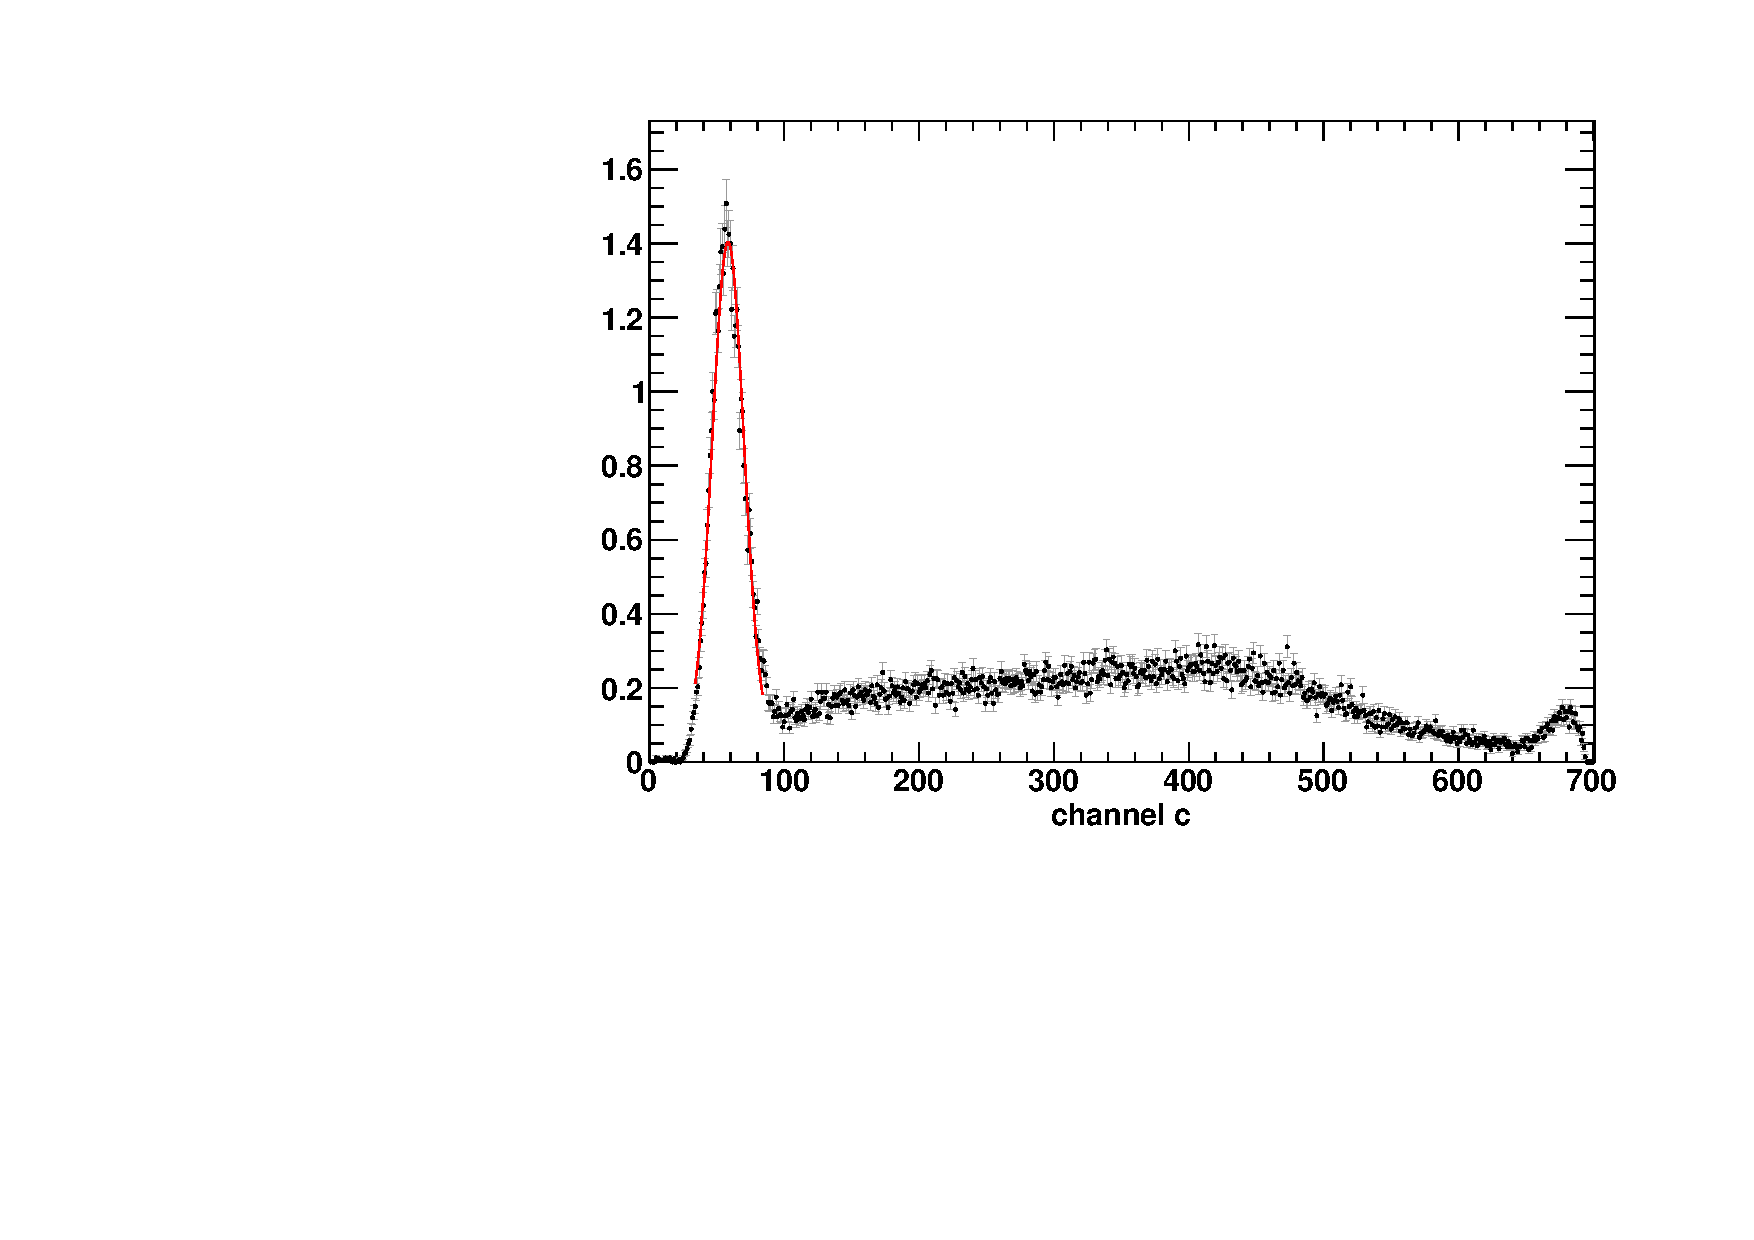
\includegraphics[width=\textwidth]{../img/energieaufloesung_059.pdf}
  \caption{Energy resolution low channal.}
  \label{img:eres:059}
\end{center}
\end{figure}

\begin{figure}[H]
\begin{center}
  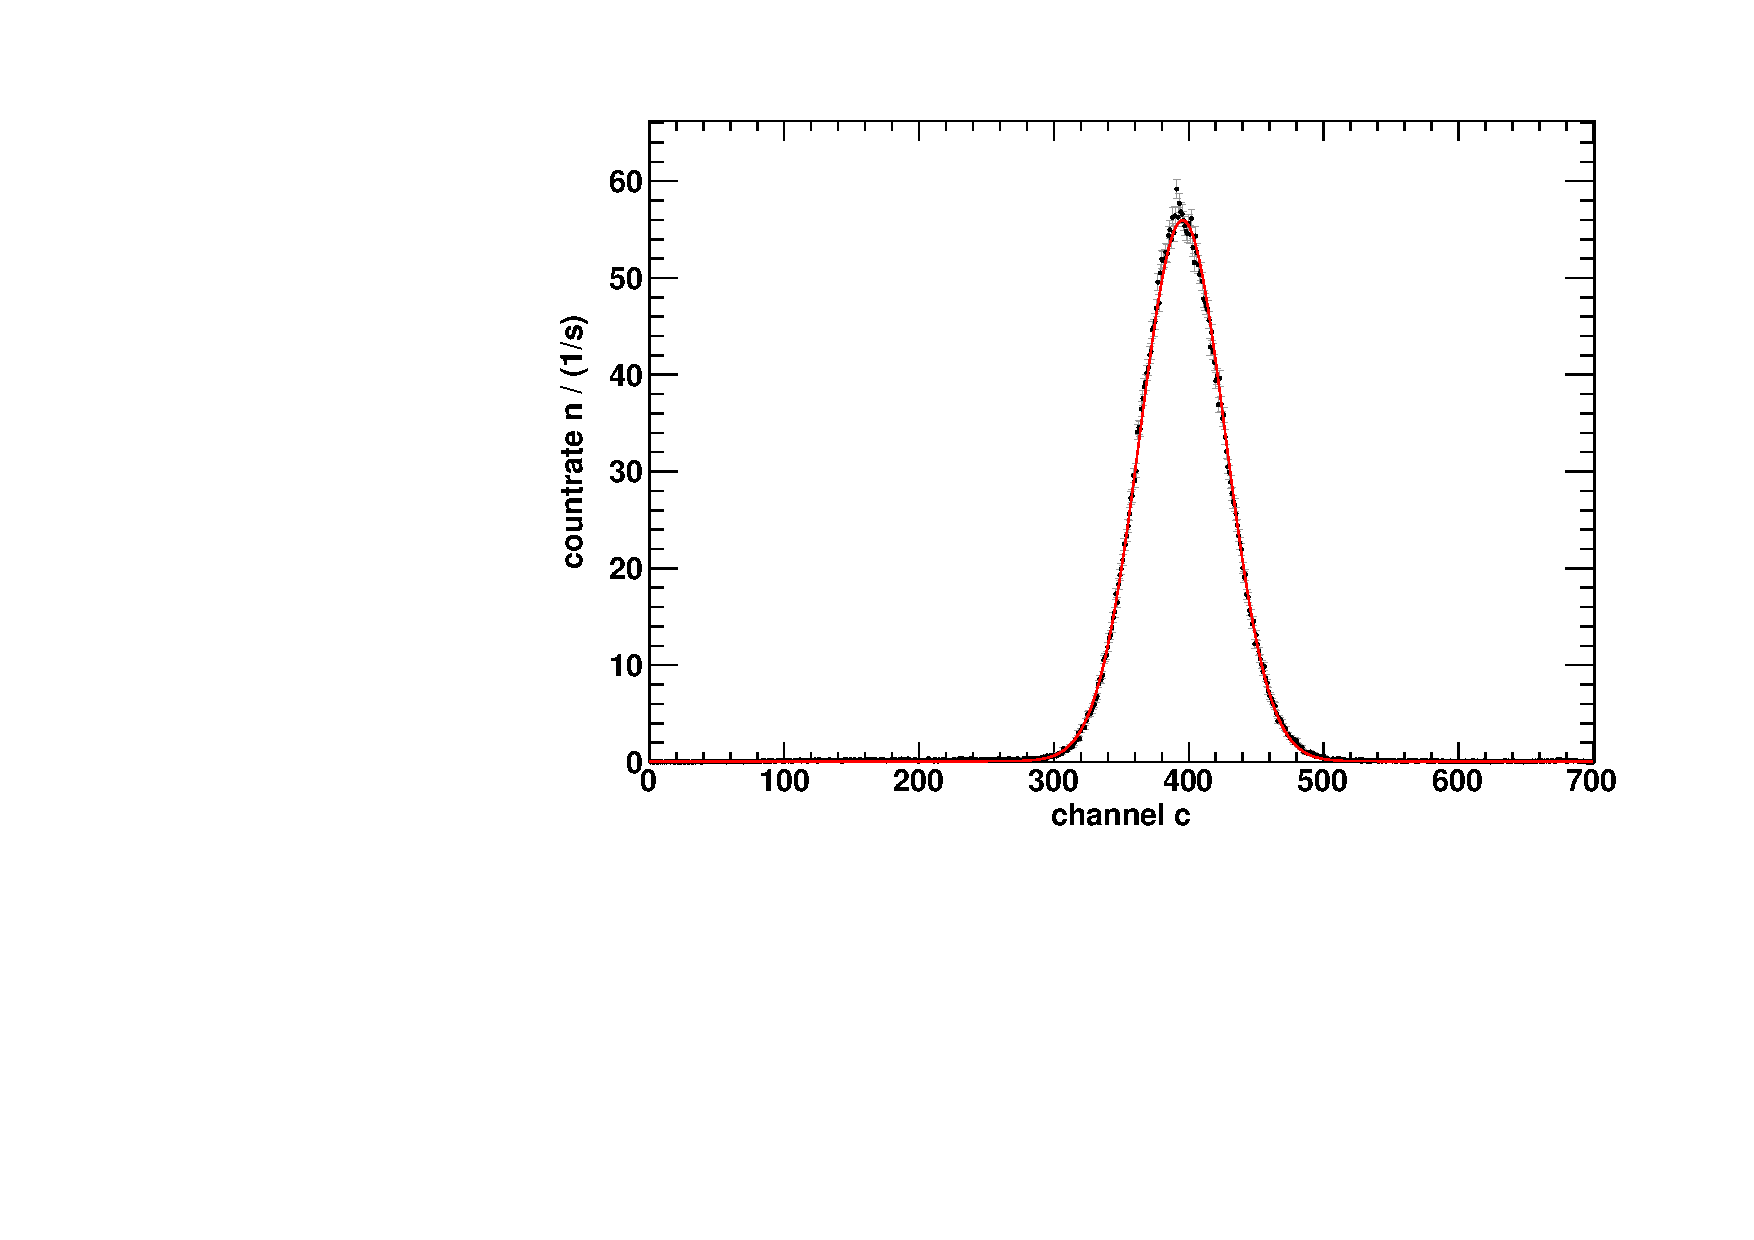
\includegraphics[width=\textwidth]{../img/energieaufloesung_400.pdf}
  \caption{Energy resolution middle channel.}
  \label{img:eres:400}
\end{center}
\end{figure}

\begin{figure}[H]
\begin{center}
  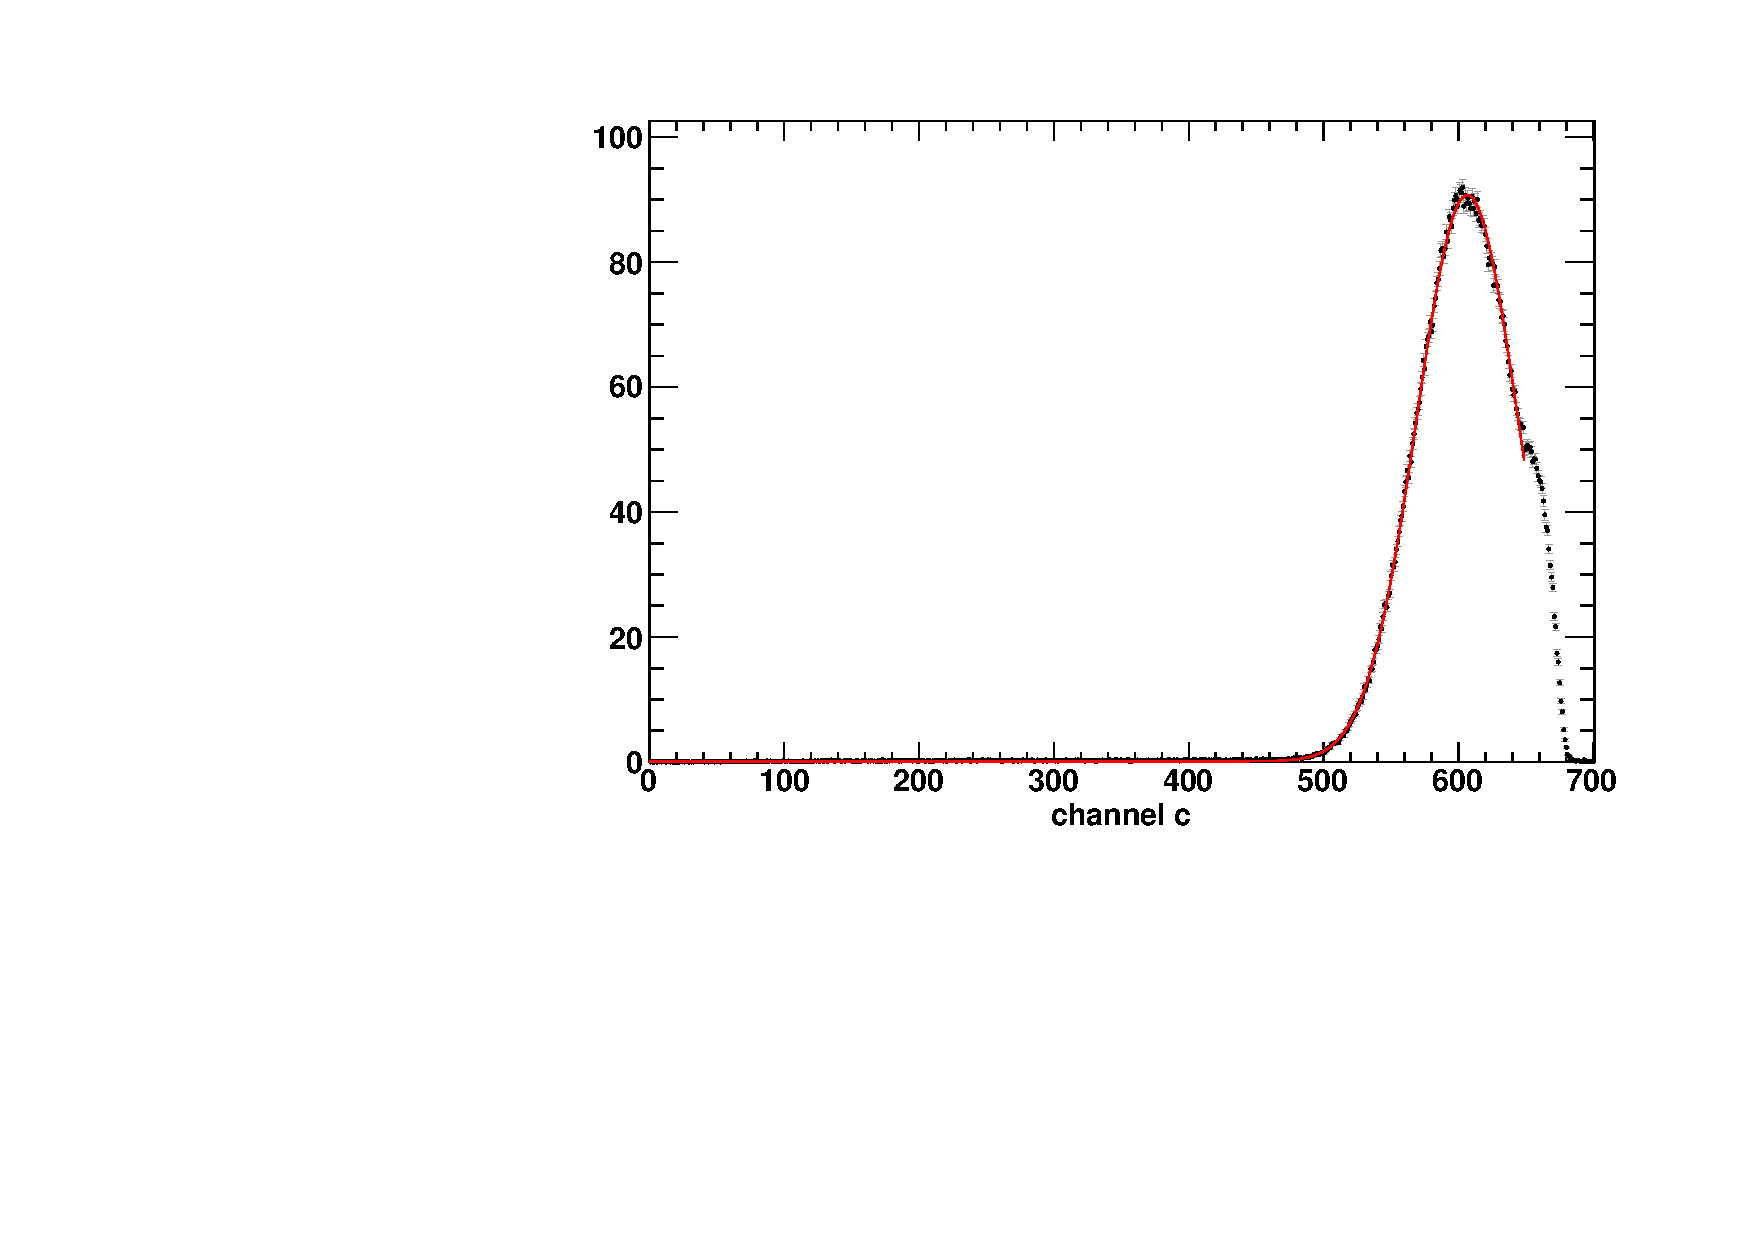
\includegraphics[width=\textwidth]{../img/energieaufloesung_604.pdf}
  \caption{Energy resolution high channel.}
  \label{img:eres:604}
\end{center}
\end{figure}

\begin{figure}[H]
\begin{center}
  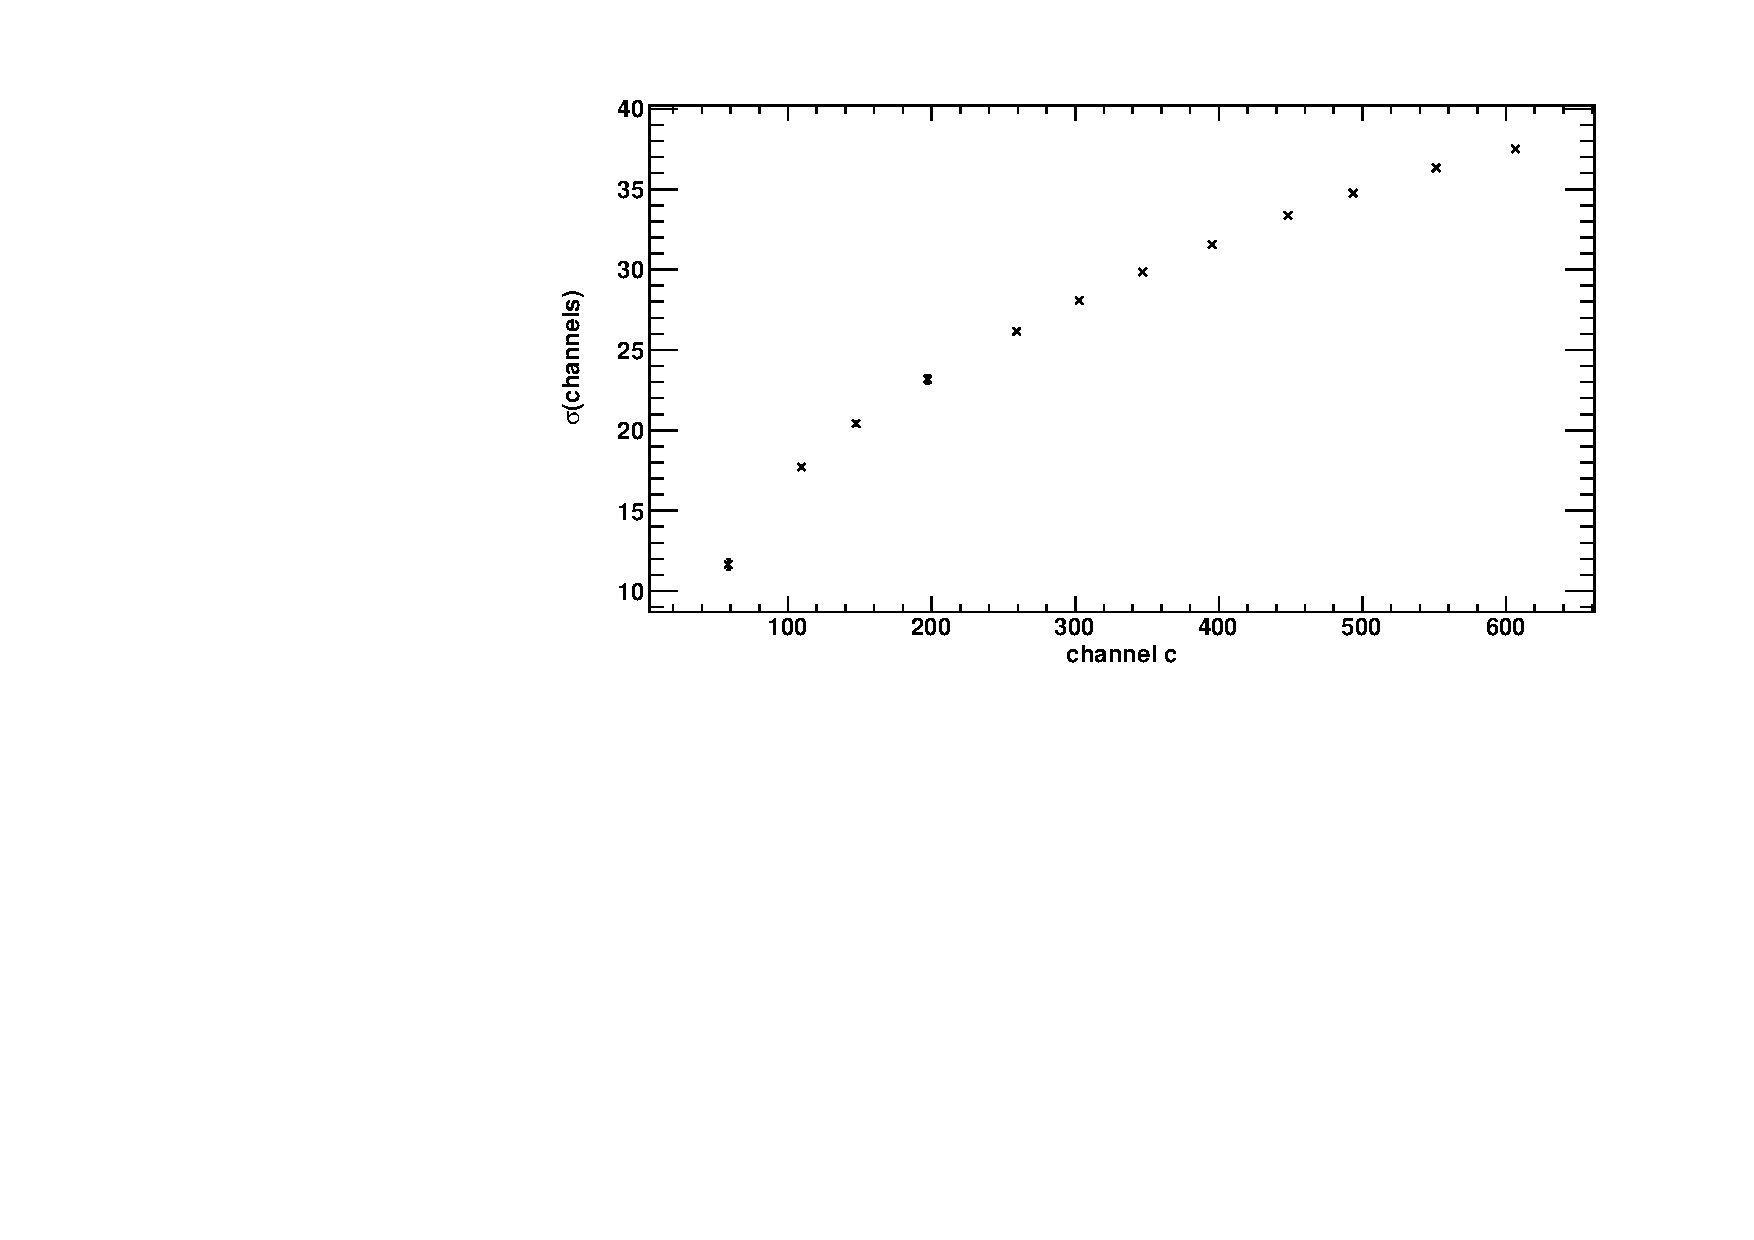
\includegraphics[width=\textwidth]{../img/energieaufloesung_channels.pdf}
  \caption{Energy resolution as a function of channels.}
  \label{img:eres:channels}
\end{center}
\end{figure}

\subsection{Energy calibration}
\subsubsection{Pedestal}
The pedestal measurement produced a Gaussian distributed spectrum (\autoref{img:pedestal})
\begin{figure}[H]
\begin{center}
  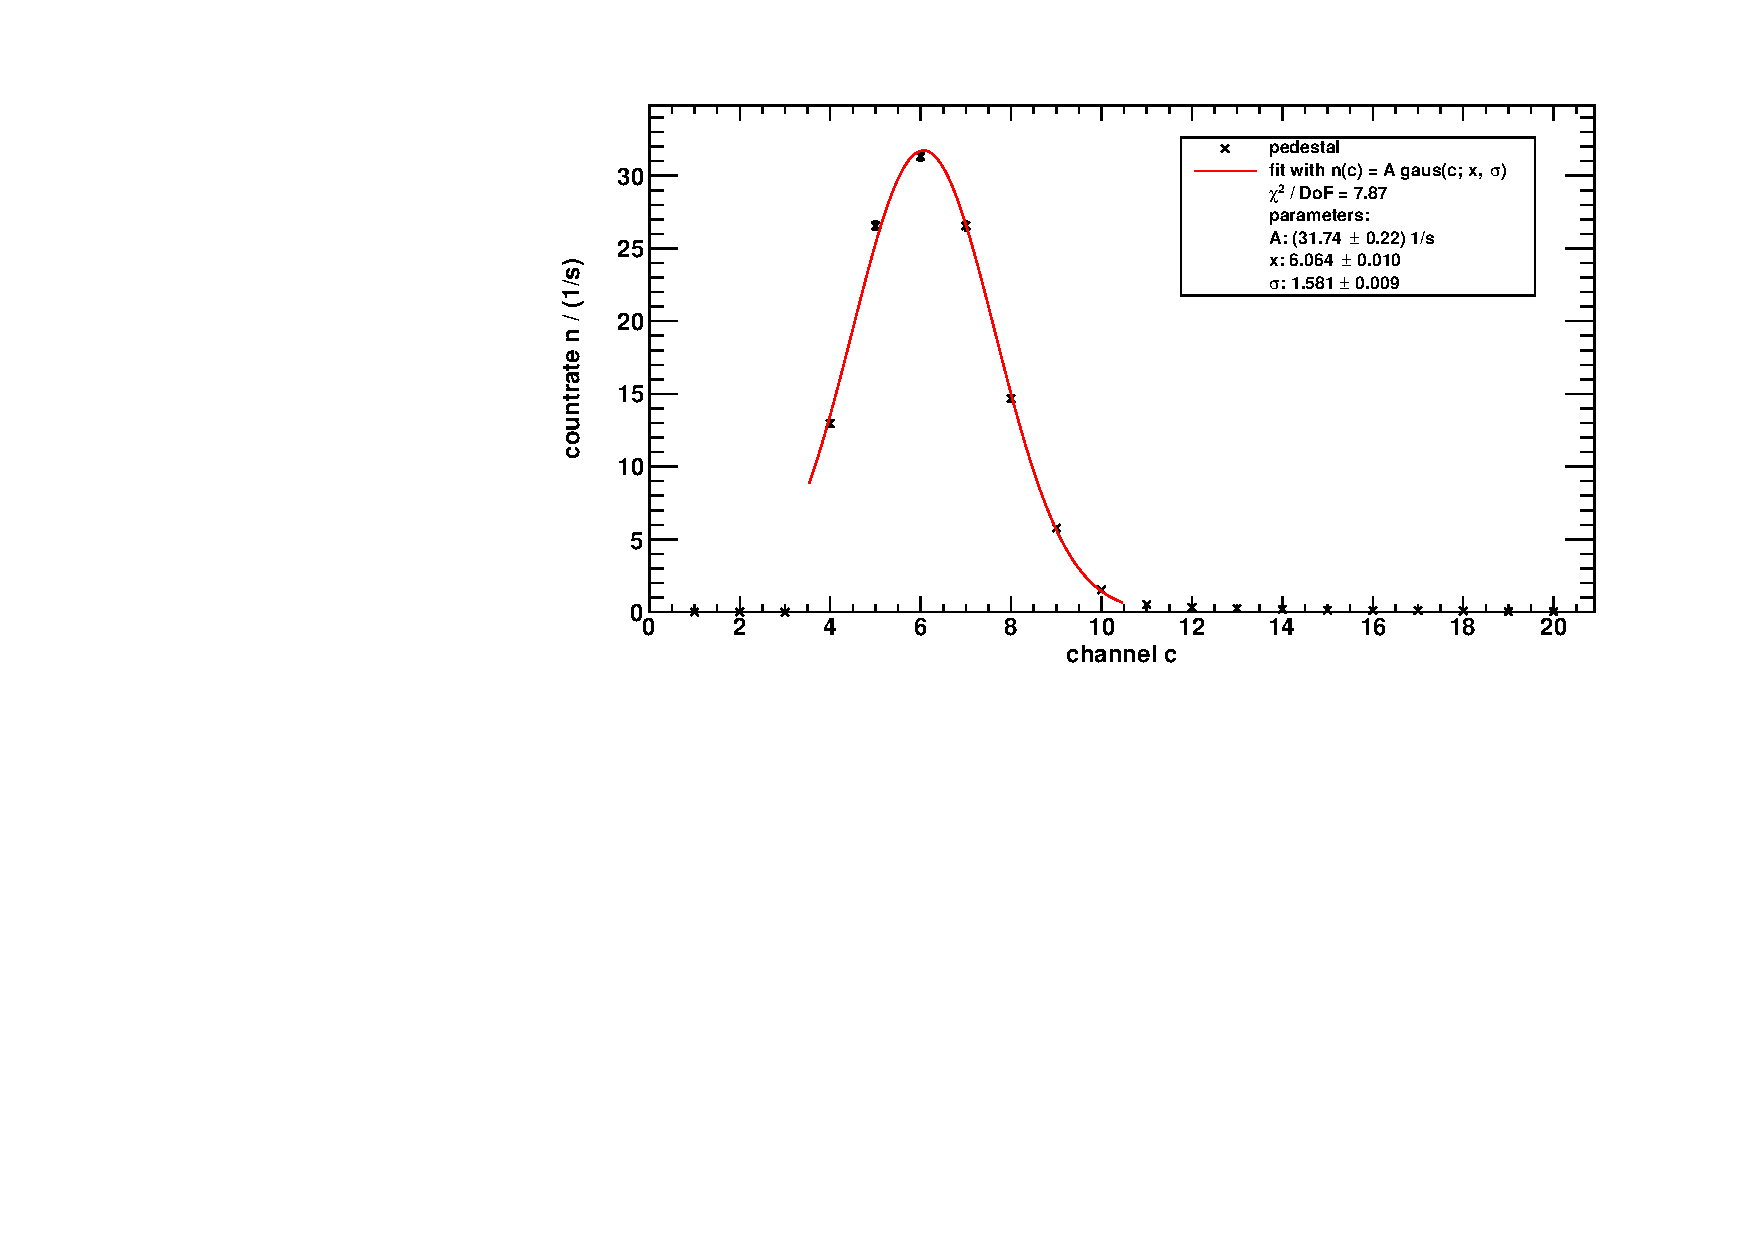
\includegraphics[width=\textwidth]{../img/pedestal.pdf}
  \caption{Pedestal.}
  \label{img:pedestal}
\end{center}
\end{figure}
The peak is fitted with the Gaussian distribution multiplied by an amplitude $A$:
\begin{equation}
    n(c) = A \cdot \gaus(c;x,\sigma)
\end{equation}
The expectation value of the fitted Gaussian distribution is:
\begin{equation}
    x = (6.064 \pm 0.010)
\end{equation}

\subsubsection{Flight through spectra}
\paragraph{Landau distribution}
The Landau distribution describes the fluctuations of energy loss caused by impact ionizatin. \\
Image Landau \\
Convolution with gaus
\begin{figure}[H]
\begin{center}
  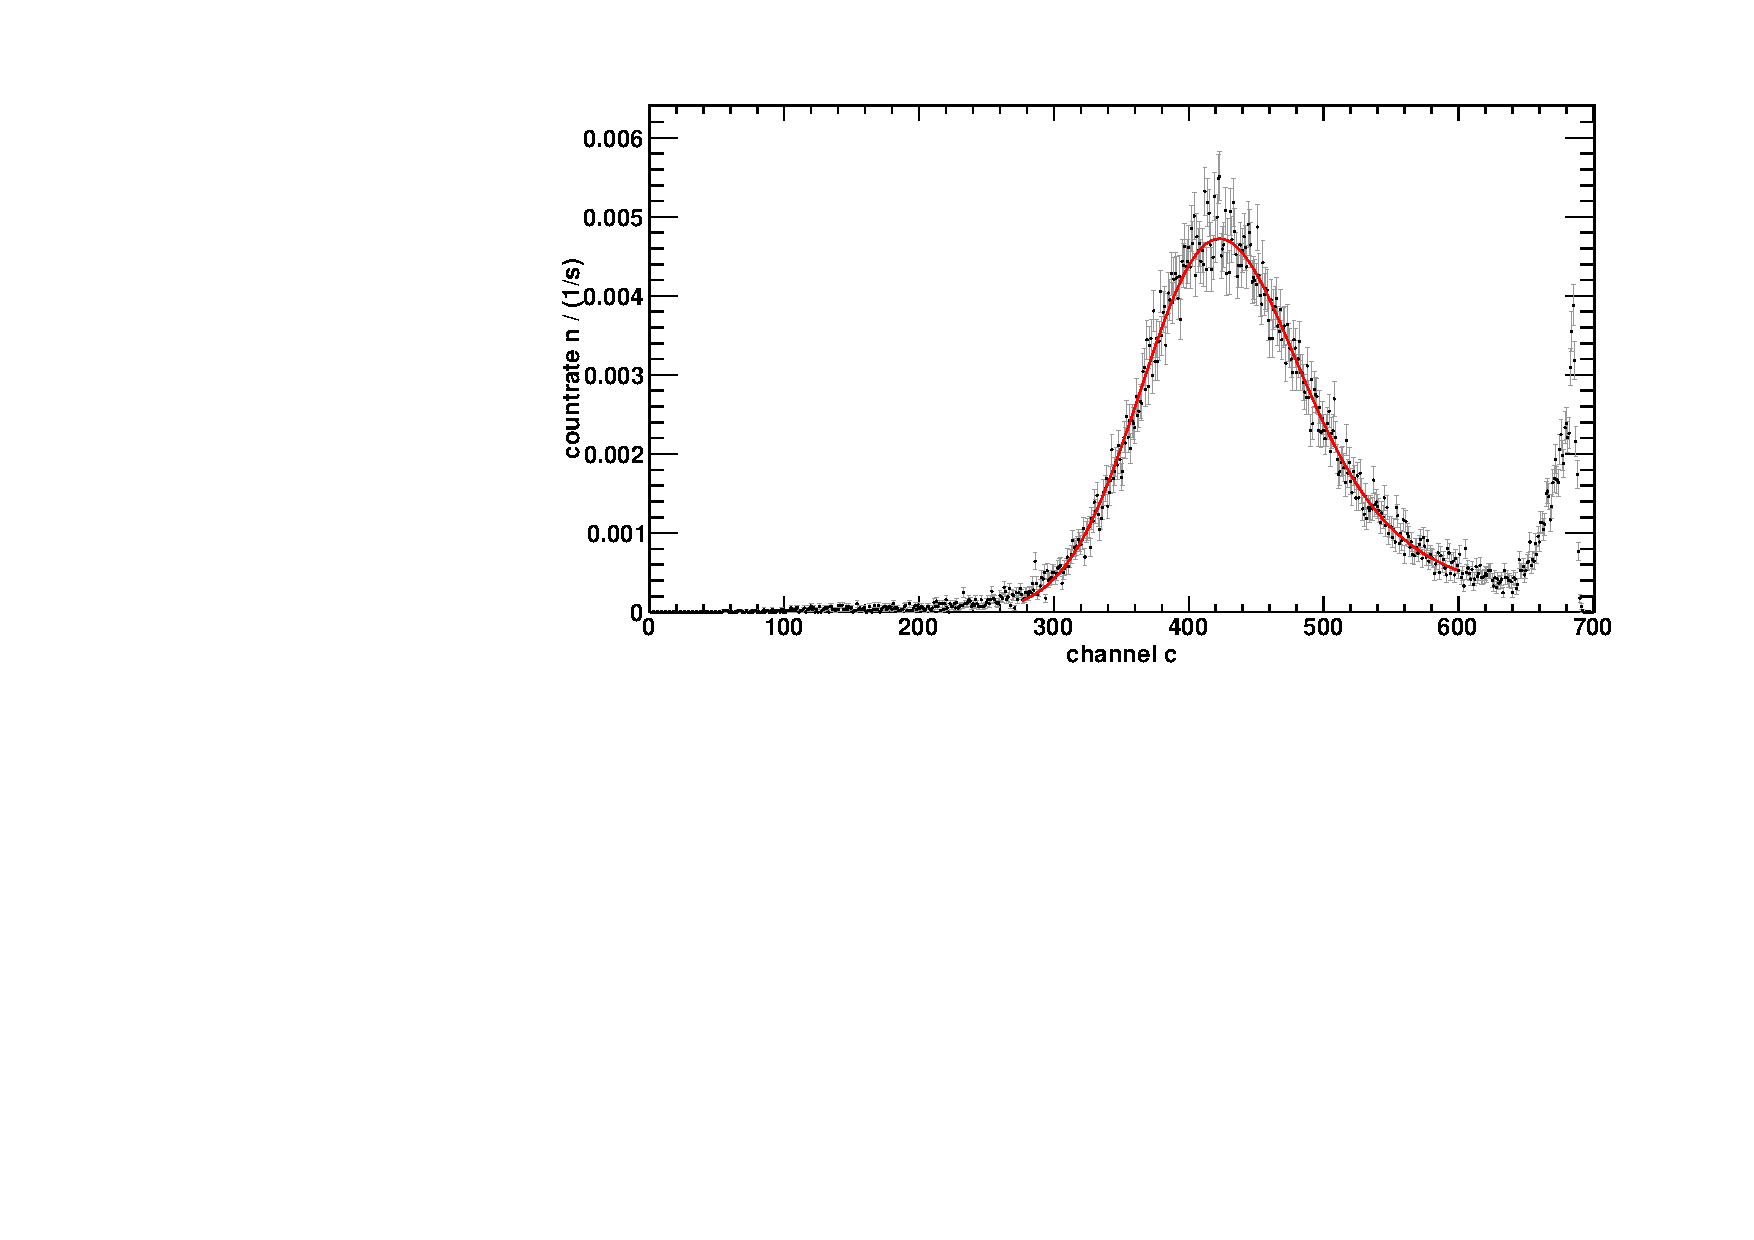
\includegraphics[width=\textwidth]{../img/energiekalibration_100.pdf}
  \caption{Flight through spectrum at 100$\%$ energy.}
  \label{img:label}
\end{center}
\end{figure}

\begin{figure}[H]
\begin{center}
  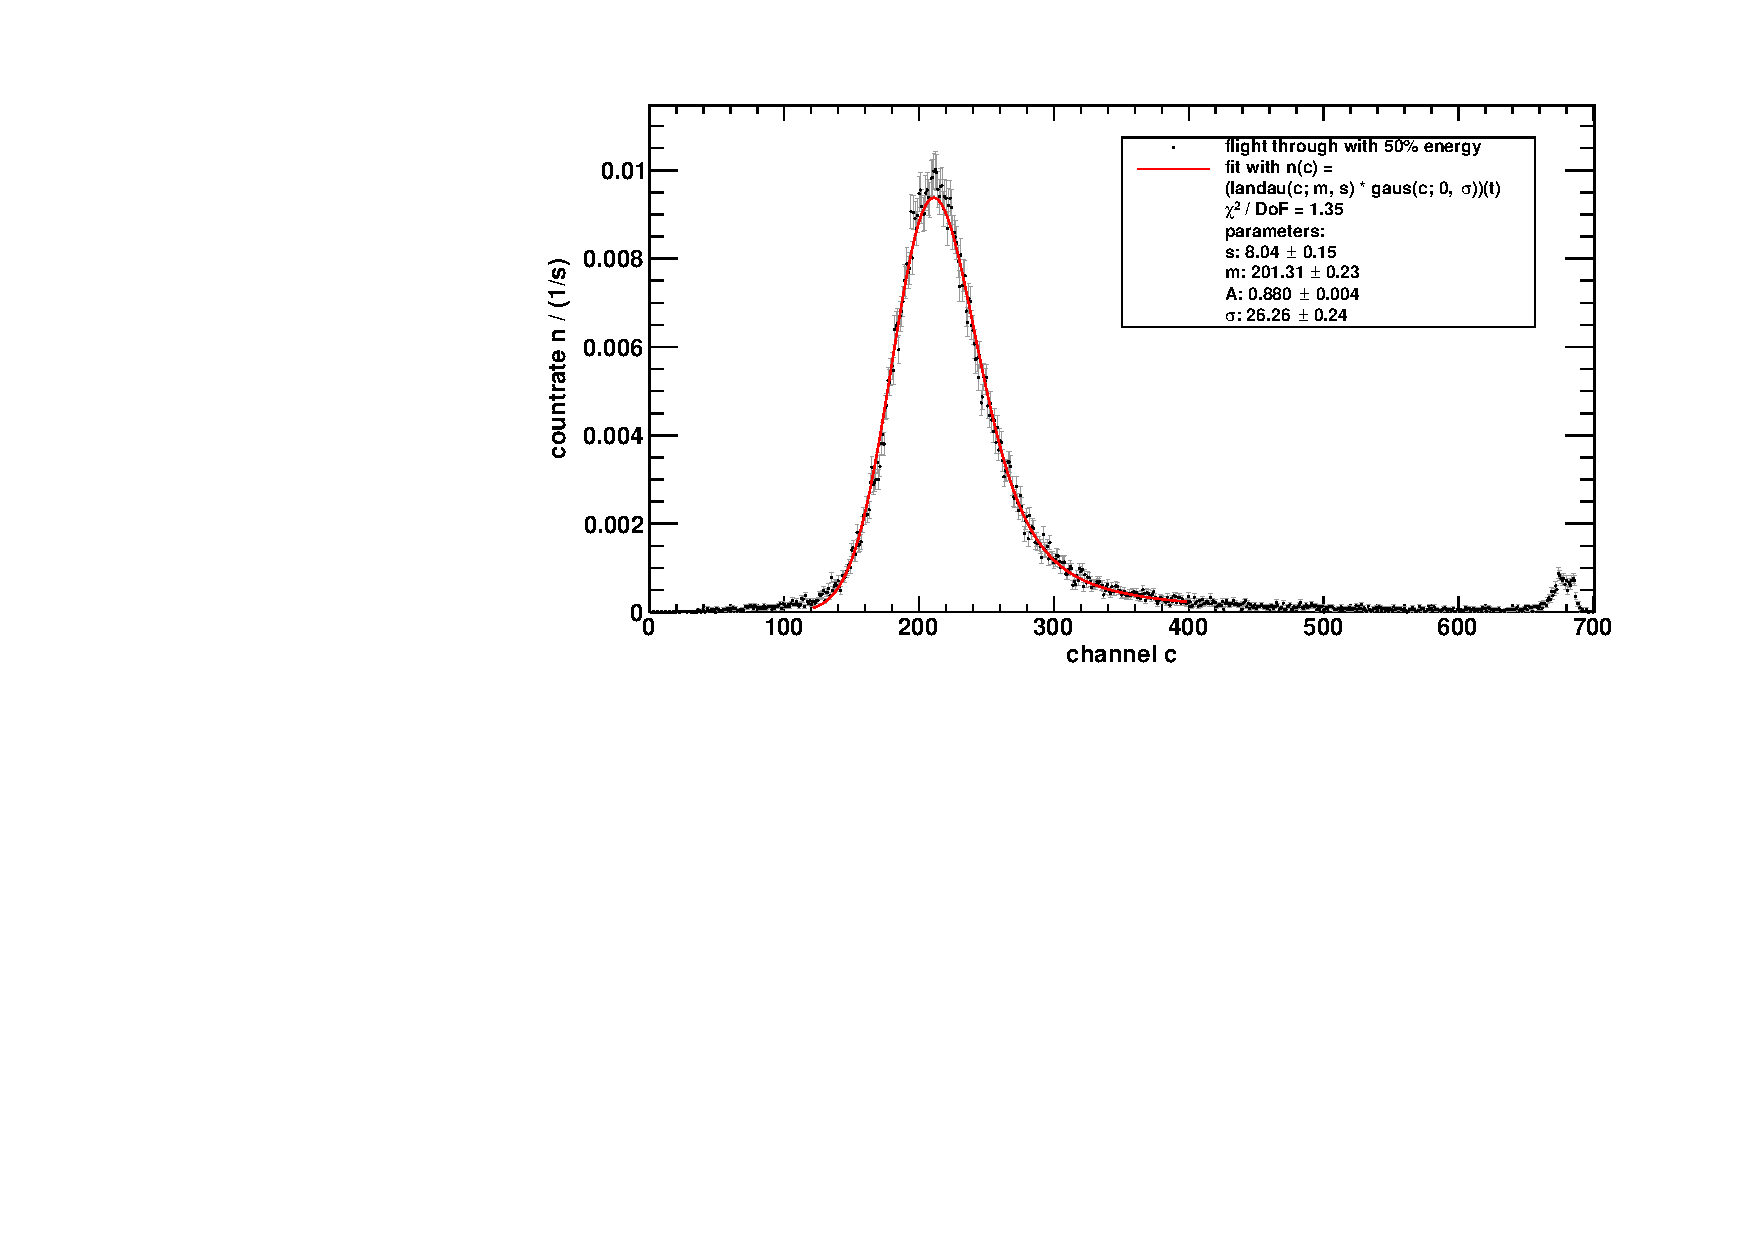
\includegraphics[width=\textwidth]{../img/energiekalibration_50.pdf}
  \caption{Flight through spectrum at 50$\%$ energy.}
  \label{img:label}
\end{center}
\end{figure}

\begin{figure}[H]
\begin{center}
  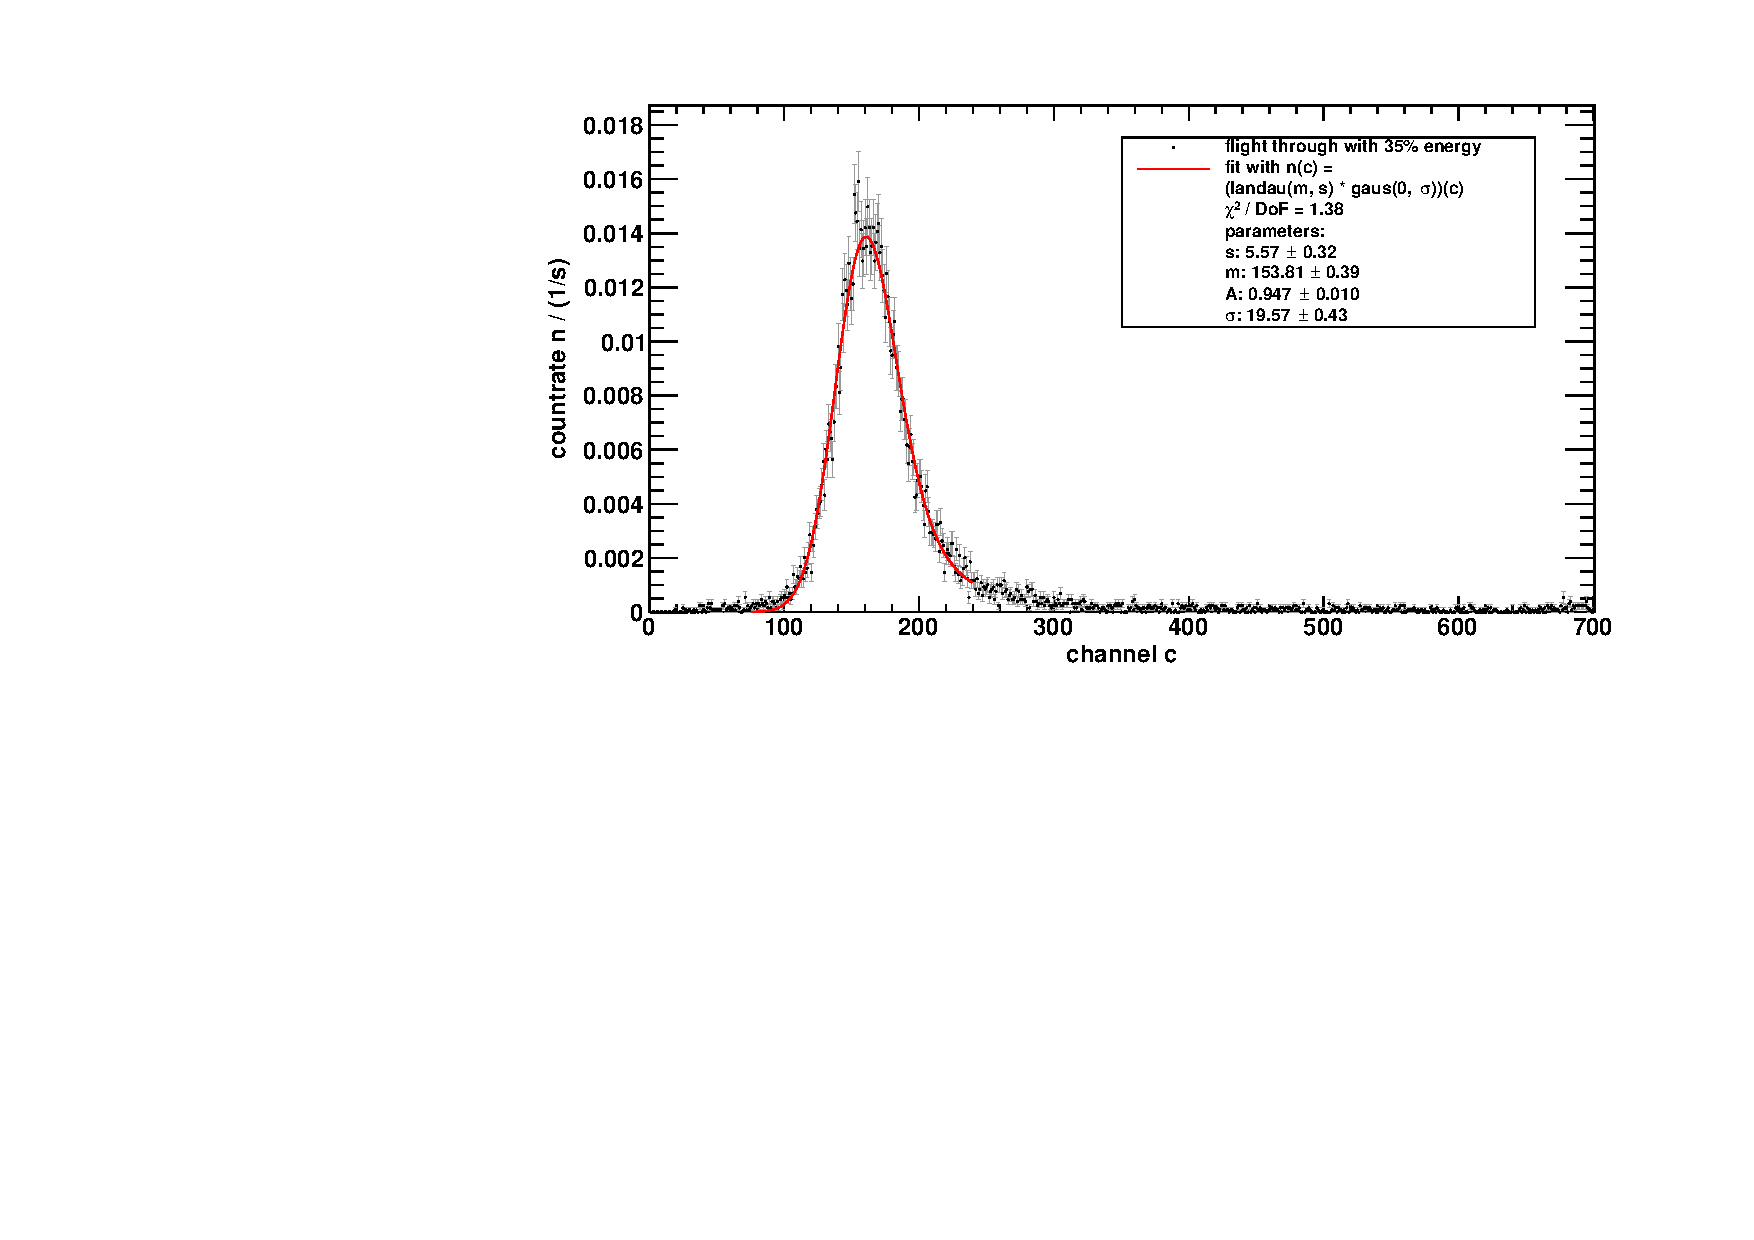
\includegraphics[width=\textwidth]{../img/energiekalibration_35.pdf}
  \caption{Flight through spectrum at 35$\%$ energy.}
  \label{img:label}
\end{center}
\end{figure}

\subsubsection{Calibration}
For the calibration it must be known, how much energy a muon deposits in the tank. Following data was given:
\begin{equation}
    \begin{split}
        & \frac{\partial E}{\partial \rho x} = (1.95 \pm 0.05)\,\frac{\text{MeV}\cdot\text{cm}^2}{\text{g}} \qquad \text{(minimal ionizing muon)}  \\
        & \rho = (0.87 \pm 0.01) \, \frac{\text{g}}{\text{cm}^3}  \qquad \qquad \qquad \text{(density of solvent)} \\
        & s = (84 \pm 5) \, \text{cm} \qquad \qquad \qquad \qquad \quad  \text{(mean free path in tank)}
    \end{split}
\end{equation}
Hence the total loss of energy calculates to:
\begin{equation}
    \begin{split}
        & E = \frac{\partial E}{\partial \rho x} \cdot \rho \cdot s = 142.5\,\text{MeV} \\
        & s_{E} = E \cdot \sqrt{ \left( \frac{s_{\frac{\partial E}{\partial \rho x}}}{\frac{\partial E}{\partial \rho x}} \right)^2 + \left( \frac{s_\rho}{\rho} \right)^2 + \left( \frac{s_s}{s} \right)^2  }
        = 9.4
    \end{split}
\end{equation}
The percentage loss of energy can now be determined:
\begin{equation}
    E_p = p \cdot E, \qquad s_{E_p} = p \cdot s_E, \qquad 0 \leq p \leq 1  %TODO Fehler auf p wegen Dämpfer?
\end{equation}
The fitted peaks of the energy calibration and their respective energies are listed in \autoref{tab:ecal} and visualized in \autoref{img:energycalibration}.
\begin{table}[H]
\caption{Channels of fitted peaks and their theoretical energy for the energy calibration.}
\begin{center}
\begin{tabular}{|c|c|c|c|c|}
  \hline
  \% energy & $c$ & $s_c$ & $E$ / MeV & $s_E$ / MeV \\ \hline
  0 & 6.064 & 0.010 & 0.0 & 0.0 \\ \hline
  35 & 153.808 & 0.392 & 49.9 & 3.0 \\ \hline
  50 & 201.312 & 0.225 & 71.3 & 4.3 \\ \hline
  100 & 404.770 & 0.547 & 142.5 & 8.5 \\ \hline
\end{tabular}
\end{center}
\label{tab:ecal}
\end{table}

\begin{figure}[H]
\begin{center}
  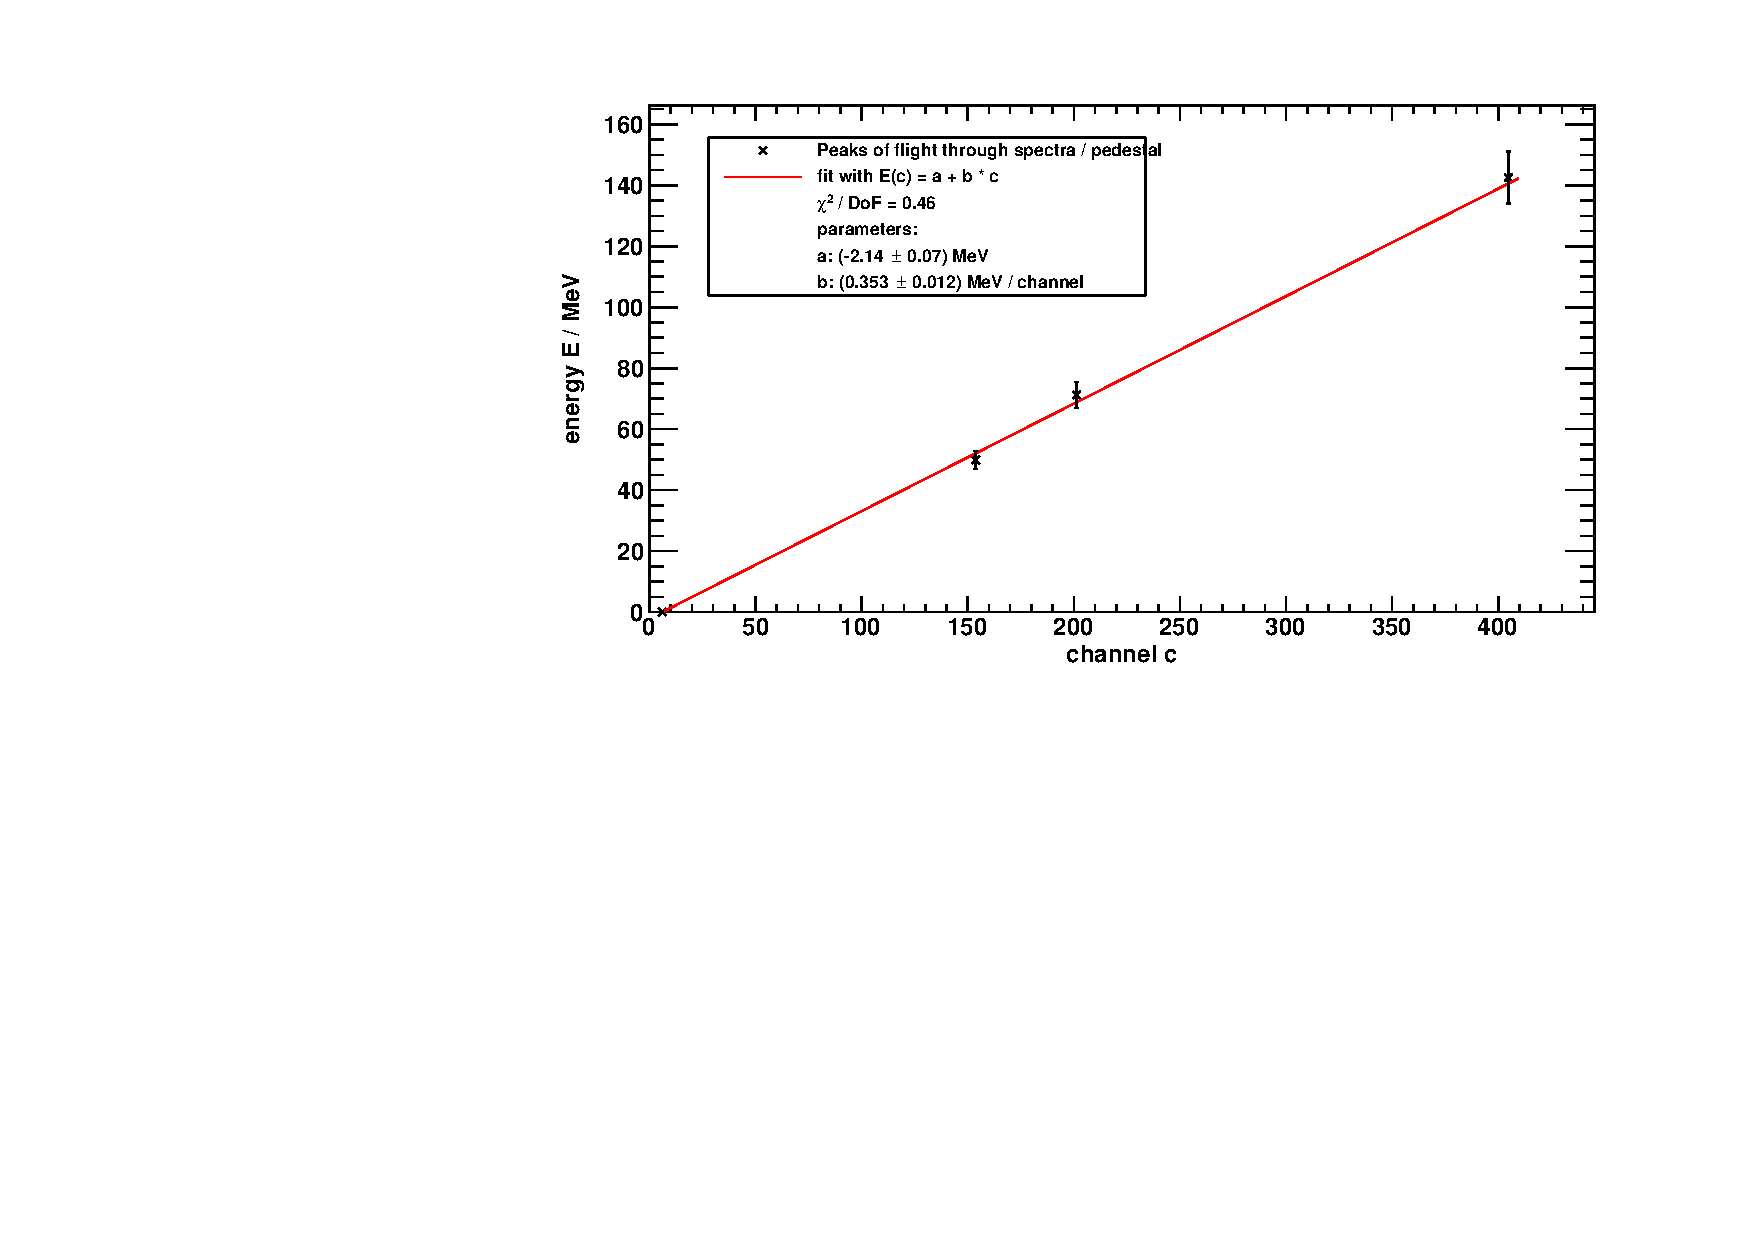
\includegraphics[width=\textwidth]{../img/energyCalibration.pdf}
  \caption{Energy calibration.}
  \label{img:energycalibration}
\end{center}
\end{figure}
Since the scintillators should produce a signal amplitude linear to the meassured energy, a linear fit is implemented:
\begin{equation}
    E(c) = a + b \cdot c
\end{equation}
The fit yields:
\begin{equation}
    \begin{split}
        & a = (-2.14 \pm 0.07) \, \text{MeV} \\
        & b = (0.353 \pm 0.012) \, \frac{\text{MeV}}{\text{channel}} \\
        & \cov(a, b) = -0.0009 \, \frac{\text{MeV}^2}{\text{channel}} 
    \end{split}
\end{equation}
Now the energy $E$ of a channel $c$ and its error $s_E$ can be calculated with:
\begin{equation}
\label{eq:ecalibration}
    E = a + b \cdot c, \qquad s_E = \sqrt{s_a^2 + \left(c \cdot s_b \right)^2 + 2 \cdot c \cdot \cov(a,b)}
\end{equation}

\subsection{Time calibration}
In \autoref{tab:tcal} the data for the time calibration is listed.
In each of the four measurements, there were only one or two channels of MCA\,II responding,
so there is no need to fit the data.
\begin{table}[H]
\caption{Measured times and channels with errors for the time calibration.}
\begin{center}
\begin{tabular}{|c|c|c|c|}
  \hline
  $t$ / \textmu s & $s_t$ / \textmu s & $c$ & $s_c$ \\ \hline
  2.40 & 0.02 & 113.0 & 0.5 \\ \hline
  4.50 & 0.02 & 223.0 & 0.5 \\ \hline
  6.25 & 0.02 & 315.5 & 0.5 \\ \hline
  8.60 & 0.02 & 441.0 & 0.5 \\ \hline
\end{tabular}
\end{center}
\label{tab:tcal}
\end{table}

A linear fit is done (\autoref{img:timecalibration}):
\begin{equation}
    t = a + b \cdot c
\end{equation}
\begin{figure}[H]
\begin{center}
  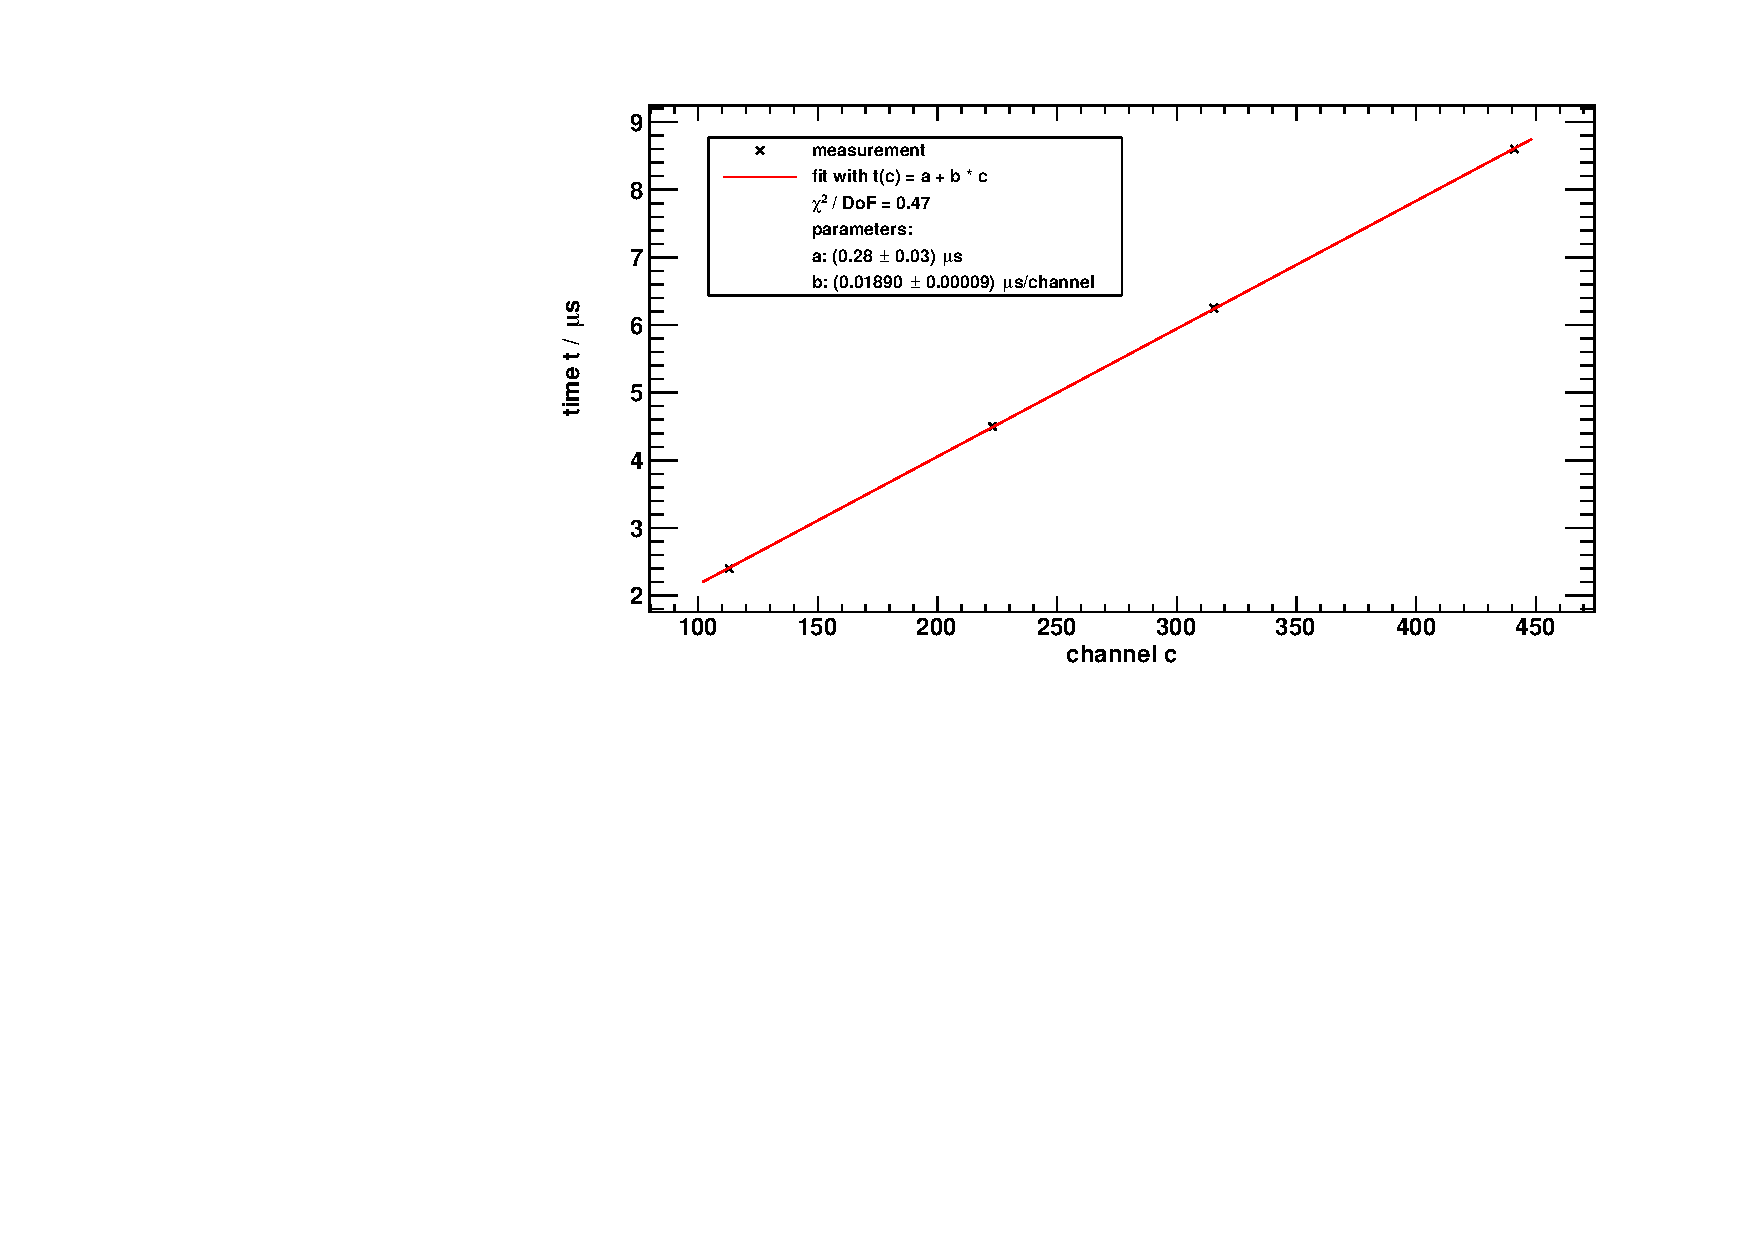
\includegraphics[width=\textwidth]{../img/timeCalibration.pdf}
  \caption{Time Calibration.}
  \label{img:timecalibration}
\end{center}
\end{figure}
The parameters and their covariance for this fit are:
\begin{equation}
    \begin{split}
        & a = (0.28 \pm 0.03) \, \text{\textmu s} \\
        & b = (0.01890 \pm 0.00009) \, \frac{\text{\textmu s}}{\text{channel}} \\
        & \cov(a, b) = -2.299 \, \frac{\text{\textmu s}^2}{\text{channel}} 
    \end{split}
\end{equation}
Now the time $t$ of a channel $c$ and its error $s_t$ can be calculated with:
\begin{equation}
\label{eq:tcalibration}
    t = a + b \cdot c, \qquad s_t = \sqrt{s_a^2 + \left(x \cdot s_b \right)^2 + 2 \cdot x \cdot \cov(a,b)}
\end{equation}

\subsection{Underground}
The underground measurement is visualized in \autoref{img:underground}.
\begin{figure}[H]
\begin{center}
  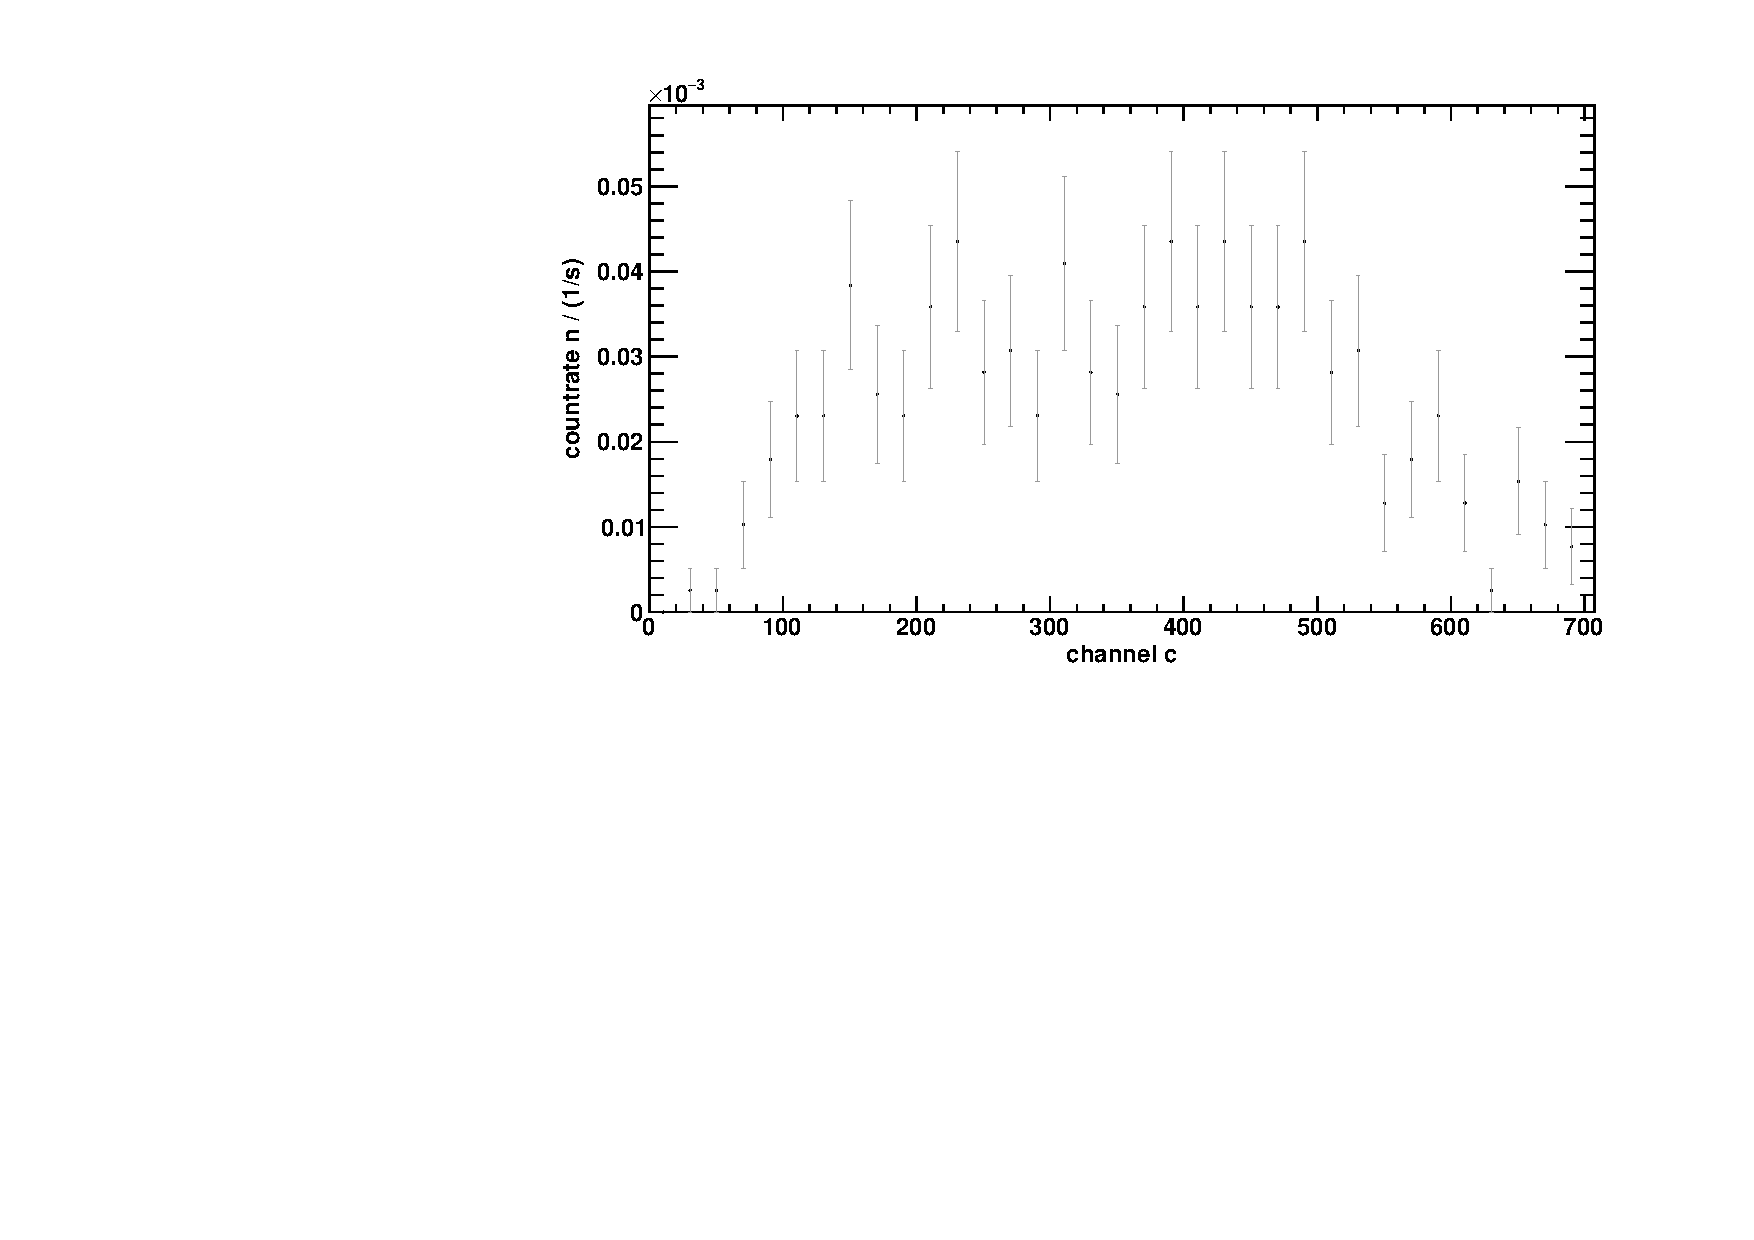
\includegraphics[width=\textwidth]{../img/underground.pdf}
  \caption{Underground.}
  \label{img:underground}
\end{center}
\end{figure}

no time underground

\subsection{\textbeta-spectrum}
The measured \textbeta-spectrum is shown in \autoref{img:beta:spectrum}.
\begin{figure}[H]
\begin{center}
  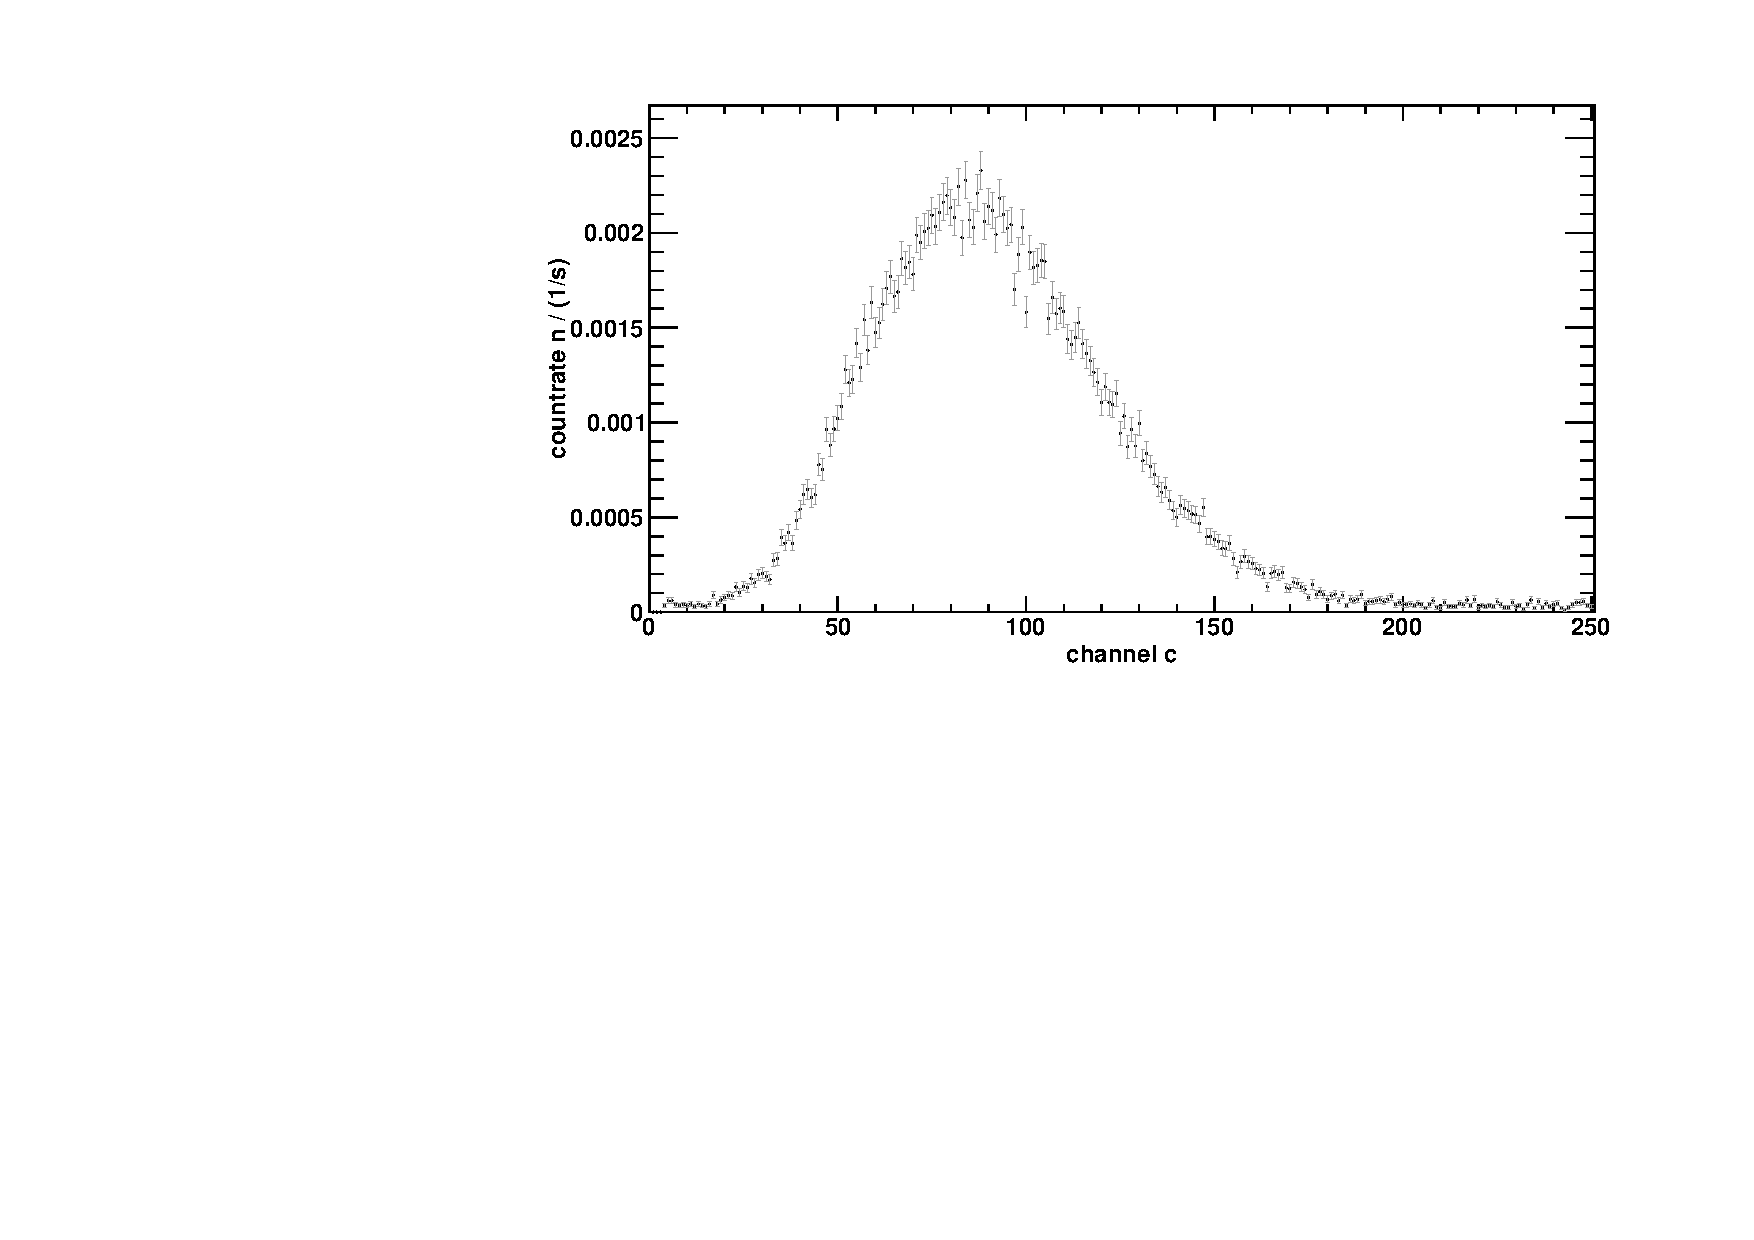
\includegraphics[width=\textwidth]{../img/betaspectrum.pdf}
  \caption{\textbeta-spectrum.}
  \label{img:beta:spectrum}
\end{center}
\end{figure}
The problem is to extract the maximal energy while taking the Gaussion blur caused by the energy resolution into account. One method is the 
\emph{Fermi-Kurie-plot} (\cite{dem4}, p.52-53).
First the channal information is converted into an energy with \autoref{eq:ecalibration}. Then $\sqrt{n(E)/E^2}$ is plotted against 
the energy $E$ (\autoref{img:beta:fermikuriefit}). Ideally a linear relationships should be identifiable. The intersection of this line with 
the $x$-axis is the maximal energy. \\
TODO warum nur teilweise linear? \\ %TODO text
The linear part gets fitted wtih
\begin{equation}
    \sqrt{n(E)/E^2} = a(E-b),
\end{equation}
so that the intersection with the $x$-axis can be read directly.
\begin{figure}[H]
\begin{center}
  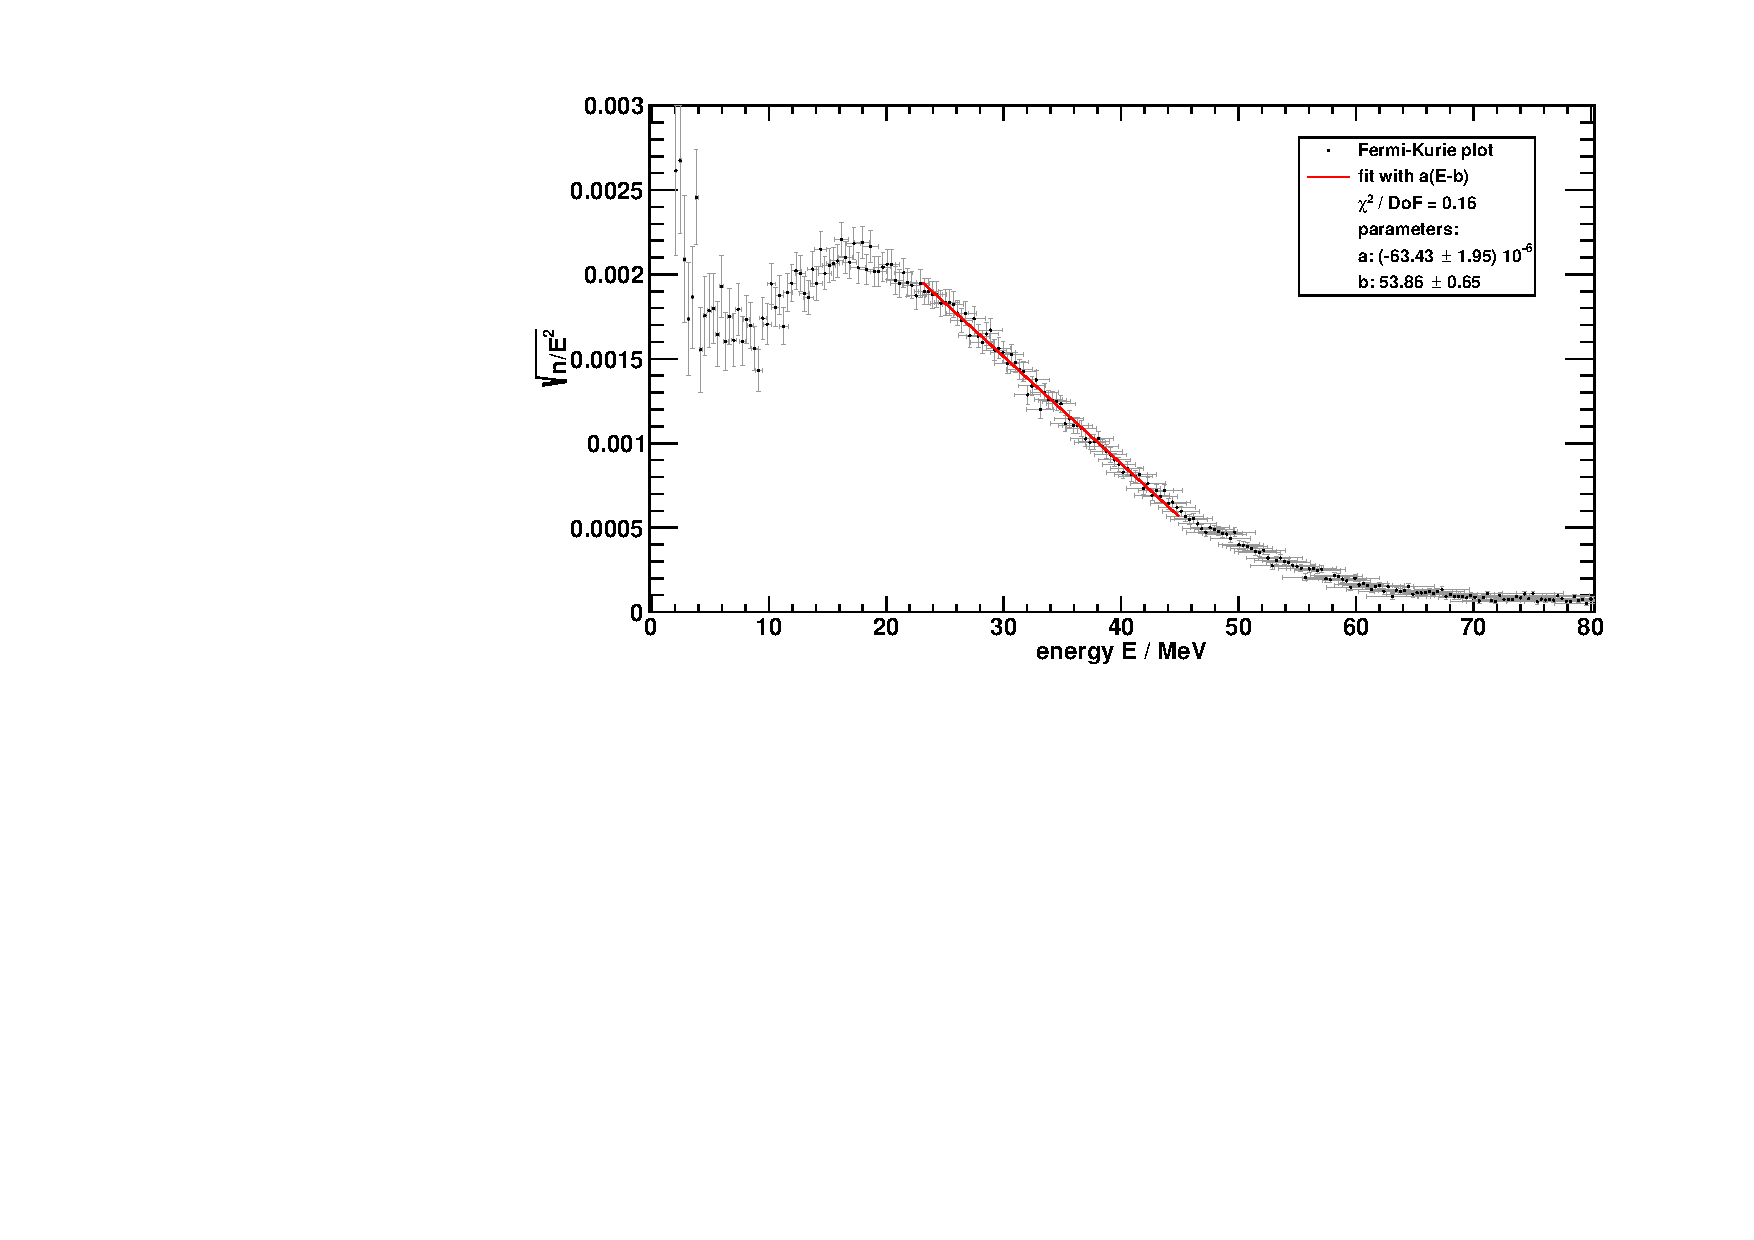
\includegraphics[width=\textwidth]{../img/betaspectrum_FermiKurie_fit.pdf}
  \caption{Fermi-Kurie plot.}
  \label{img:beta:fermikuriefit}
\end{center}
\end{figure}
With the fit one gets for $b$:
\begin{equation}
    b = (53.86 \pm 0.65)\,\text{MeV}
\end{equation}
Since this energy is half of the rest energy of the muon it has to be multiplied with 2:
\begin{equation}
\begin{split}
    & E_\mu = 2 \cdot b, \qquad s_{E_\mu} = 2 \cdot s_b \\
    & \Rightarrow E_\mu = (107.7 \pm 1.3)\,\text{MeV}
    \end{split}
\end{equation}
The so calculated rest energy matches the literature value within a 2-\textsigma-interval.
\begin{equation}
    E_\mu^{\text{lit.}} = (105.6583715 \pm 0.0000035)\,\text{MeV}
\end{equation}

\subsection{Mean lifetime}
To calculate the mean lifetime $\tau$ of $\mu$ the channels are converted to a time with \autoref{eq:tcalibration}. 
Furthermore we rebin the spectrum to get a nicer curve. Three successive channels are averaged:
\begin{equation}
    \bar{t}_i = \frac{1}{3} \sum_{j=0}^{2} t_{3i+j}, \qquad \bar{n}_i = \frac{1}{3} \sum_{j=0}^{2} n_{3i+j}, \qquad i \in \left[1, \frac{\#(t_i)}{3} \right]
\end{equation}
where $(t_i, n_i)$ are the old values and $(\bar{t}_i, \bar{n}_i)$ are the new ones. $\#(t_i)$ is the number of old values.
The errors are calculated with error propagation:
\begin{equation}
    s_{\bar{t}_i} = \frac{1}{3} \sqrt{\sum_{j=0}^{2} t_{3i+j}^2}, \qquad s_{\bar{n}_i} = \frac{1}{3} \sqrt{\sum_{j=0}^{2} n_{3i+j}^2}
\end{equation}
\begin{figure}[H]
\begin{center}
  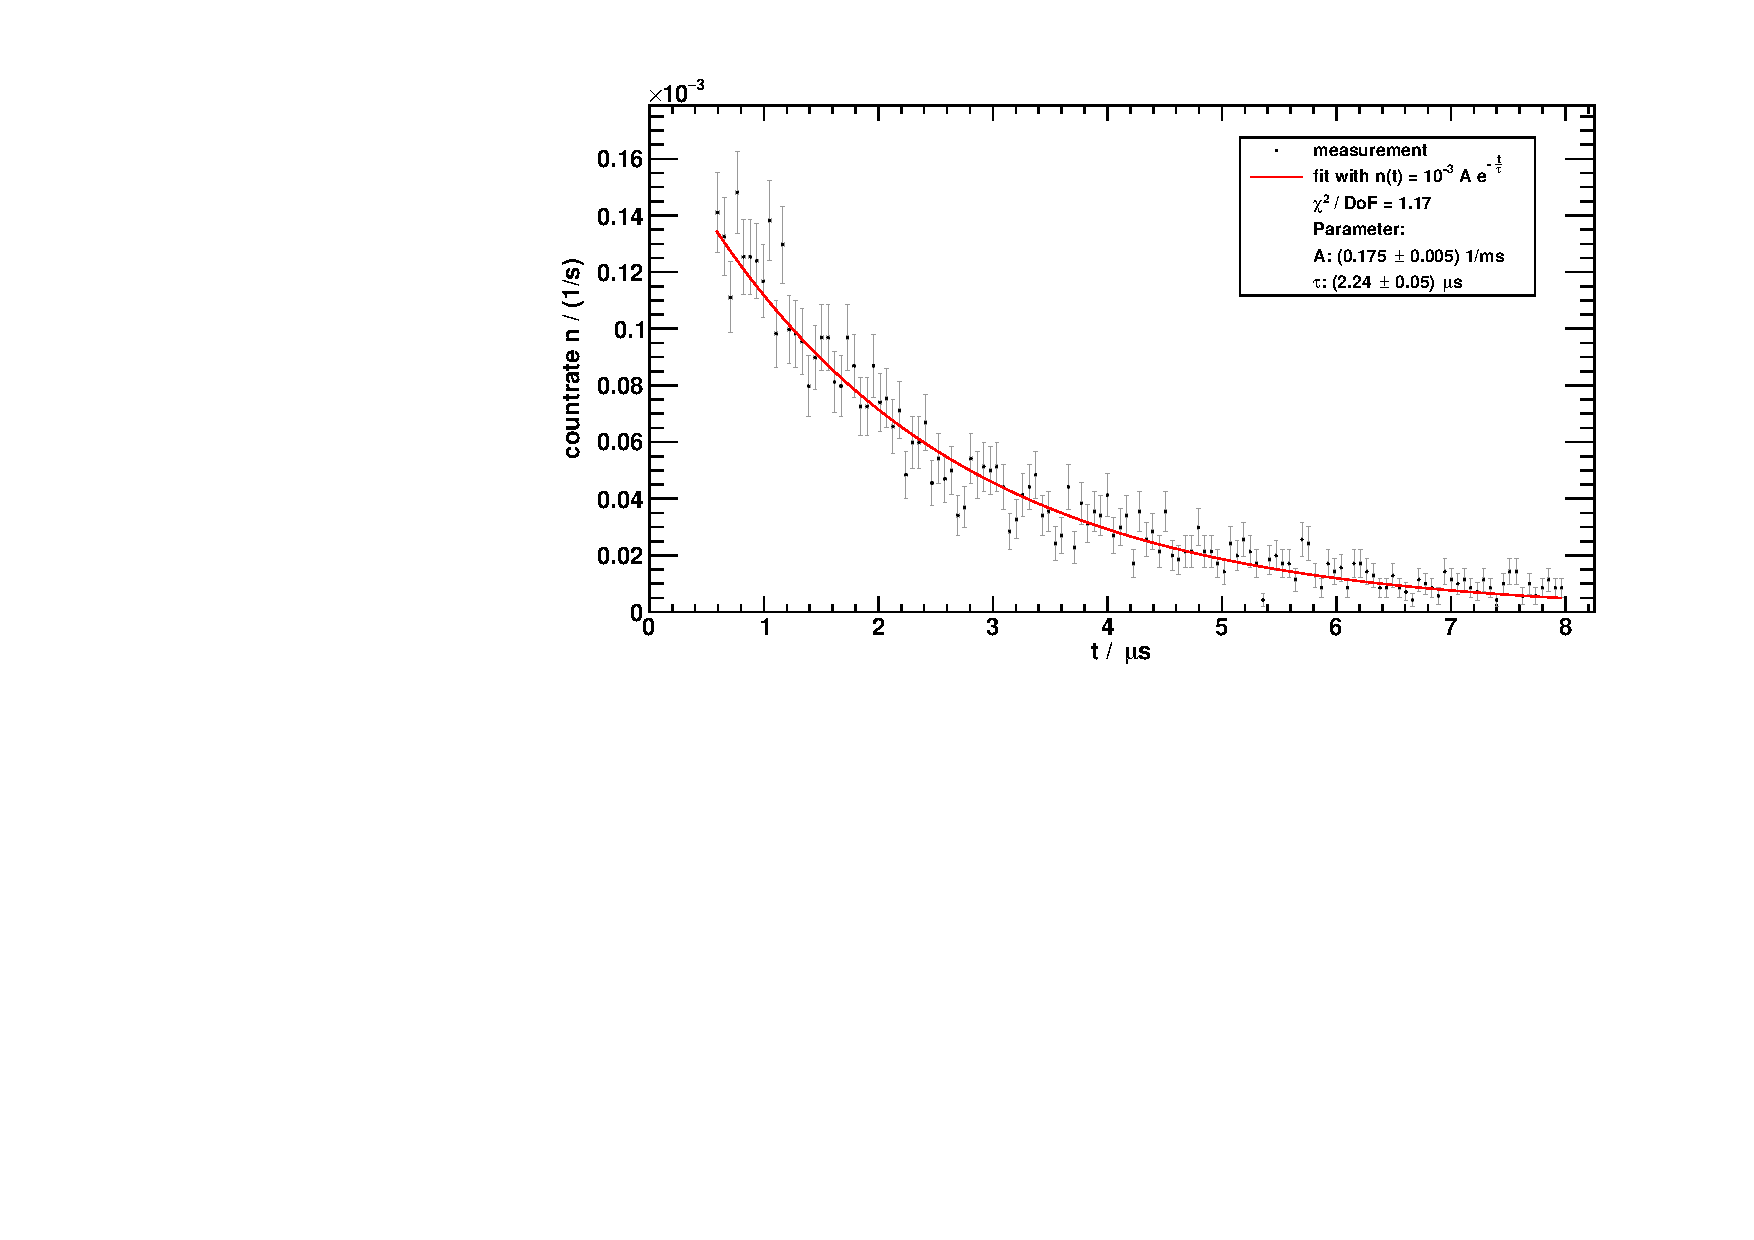
\includegraphics[width=\textwidth]{../img/decayTime.pdf}
  \caption{decay time, t-errors not visible.}
  \label{img:decaytime}
\end{center}
\end{figure}

The so obtained datapoints (\autoref{img:decaytime}) get fitted with an exponential function, since they obey the law of decay (\ref{sub:decay}):
\begin{equation}
    n = A \cdot e^{-\frac{t}{\tau}}
\end{equation}
The fit yields for the mean lifetime:
\begin{equation}
    \tau = \left( 2.24 \pm 0.05 \right)\,\text{\textmu s}
\end{equation}
This matches with the literature value within 1-\textsigma-interval. %TODO ref lit value
\begin{equation}
    \tau^{\text{lit.}} = \left( 2.1969811 \pm 0.0000022 \right)\,\text{\textmu s}
\end{equation}

\subsection{Weak coupling constant}
\begin{equation}
    \begin{split}
        G &= \sqrt{\frac{192 \pi^2}{\tau m_\mu^5}} \\
        s_G &= \frac{1}{2} \sqrt{\frac{192 \pi^3 \left( m_\mu^2 s_\tau^2 + 25 \tau^2 s_{m_\mu}^2 \right)}{m_\mu^7 \tau^3}}
    \end{split}
\end{equation}
\begin{equation}
    G = (1.10 \pm 0.04) \cdot 10^{-5} \frac{1}{\text{GeV}^2}
\end{equation}